\documentclass[tikz,border=6pt]{standalone}
\usepackage[T1]{fontenc}
\usepackage[utf8]{inputenc}
\usepackage{pgfplots}
\usepgfplotslibrary{groupplots}
\usetikzlibrary{calc}
\pgfplotsset{compat=1.18}
\begin{document}
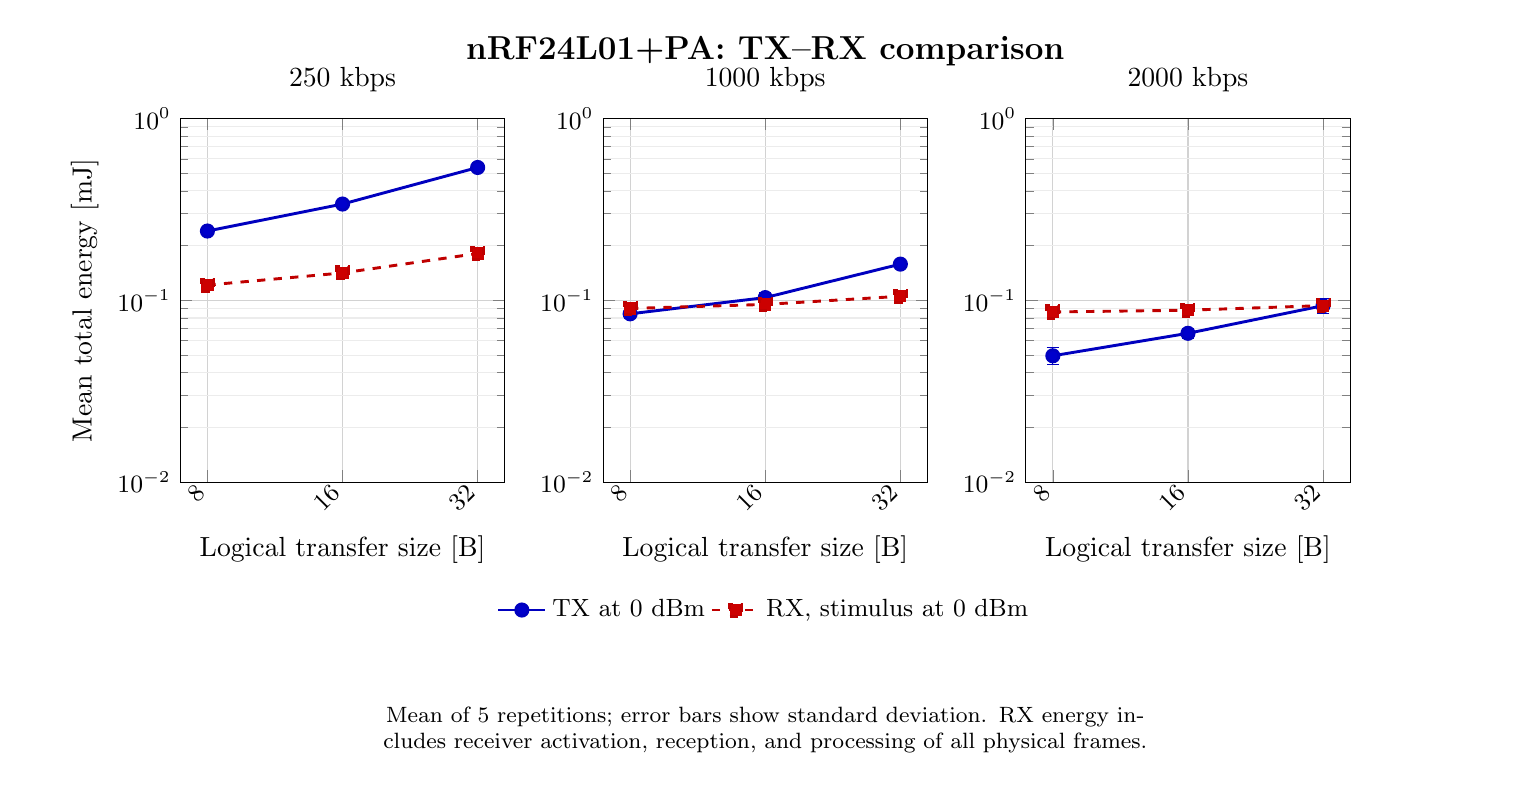
\begin{tikzpicture}
\begin{groupplot}[/pgf/number format/use comma,
  group style={group size=3 by 1, horizontal sep=1.25cm},
  width=5.7cm, height=6.2cm,
  xmode=log, log basis x={2}, ymode=log, log basis y={10},
  ymin=0.01, ymax=1,
  xtick={8,16,32}, xticklabels={8,16,32},
  x tick label style={rotate=45, anchor=east, font=\small},
  y tick label style={font=\small},
  grid=both, minor grid style={gray!15}, major grid style={gray!35},
  xlabel={Logical transfer size [B]},
  every axis plot/.append style={line width=1.05pt},
  error bars/error bar style={line width=0.35pt},
  legend style={font=\small, draw=none, fill=none, at={(0.5,-0.29)},
    anchor=north, legend columns=-1},
]
\nextgroupplot[title={250 kbps}, ylabel={Mean total energy [mJ]}]
\addplot+[color=blue!75!black, solid, mark=*, mark size=2.2pt,
  error bars/.cd, y dir=both, y explicit,
] coordinates {
  (8,0.240757209) +- (0,0.00285552535)
  (16,0.338846214) +- (0,0.0019304071)
  (32,0.538376496) +- (0,0.00213679928)
};
\addplot+[color=red!75!black, dashed, mark=square*, mark size=2.2pt,
  error bars/.cd, y dir=both, y explicit,
] coordinates {
  (8,0.121466746) +- (0,9.97063141e-05)
  (16,0.141633879) +- (0,5.57851634e-05)
  (32,0.181157847) +- (0,0.000232805431)
};
\nextgroupplot[title={1000 kbps}]
\addplot+[color=blue!75!black, solid, mark=*, mark size=2.2pt,
  error bars/.cd, y dir=both, y explicit,
] coordinates {
  (8,0.0843866627) +- (0,0.00496314984)
  (16,0.103627102) +- (0,0.00632496032)
  (32,0.158349521) +- (0,0.00454069624)
};
\addlegendentry{TX at 0 dBm}
\addplot+[color=red!75!black, dashed, mark=square*, mark size=2.2pt,
  error bars/.cd, y dir=both, y explicit,
] coordinates {
  (8,0.0902940723) +- (0,3.02141608e-05)
  (16,0.0950547443) +- (0,0.000110659849)
  (32,0.105377881) +- (0,0.000103568303)
};
\addlegendentry{RX, stimulus at 0 dBm}
\nextgroupplot[title={2000 kbps}]
\addplot+[color=blue!75!black, solid, mark=*, mark size=2.2pt,
  error bars/.cd, y dir=both, y explicit,
] coordinates {
  (8,0.0495938279) +- (0,0.00535509862)
  (16,0.0659304848) +- (0,0.00400478031)
  (32,0.0935441755) +- (0,0.00852946989)
};
\addplot+[color=red!75!black, dashed, mark=square*, mark size=2.2pt,
  error bars/.cd, y dir=both, y explicit,
] coordinates {
  (8,0.0863797362) +- (0,7.32977989e-05)
  (16,0.088355305) +- (0,0.000876368832)
  (32,0.0936585548) +- (0,7.80953303e-05)
};
\end{groupplot}
\node[font=\bfseries\large] at ($(group c2r1.north)+(0,0.85cm)$)
  {nRF24L01+PA: TX--RX comparison};
\node[font=\footnotesize, align=center, text width=18.5cm]
  at ($(group c2r1.south)+(0,-3.15cm)$)
  {Mean of 5 repetitions; error bars show standard deviation. RX energy includes receiver activation, reception, and processing of all physical frames.};
\end{tikzpicture}
\end{document}
